\documentclass[12pt]{article}
\usepackage[utf8]{inputenc}

\usepackage[margin = 0.7in]{geometry}
\usepackage{amsmath}
\usepackage{amsfonts}
\usepackage{amssymb}
\usepackage{amsthm}
\usepackage{graphicx}
\usepackage{placeins}
\usepackage{enumitem}
\usepackage{dsfont}
\usepackage{booktabs}
\usepackage{subcaption}

\newcommand{\N}{\mathbb{N}}
\newcommand{\Z}{\mathbb{Z}}
\newcommand{\R}{\mathbb{R}}
\newcommand{\E}{\mathbb{E}}
\newcommand{\Q}{\mathbb{Q}}
\newcommand{\de}{\mathrm{d}}
\newcommand{\one}{\mathds{1}}

\title{ECON 899: Problem Set 6}
\author{Katherine Kwok\footnote{I collaborated with Anya Tarascina and Claire Kim on this assignment.}}
\date{November 2021}

\begin{document}

\maketitle
\noindent \textbf{Overview:} For this assignment, the goal is to use the Hopenhayn and Rogerson (1993) algorithm to solve the equilibrium model for firm dynamics. \\\\
\noindent \textbf{Tasks:} We solve several different versions of the Hopenhayn and Rogerson (1993) model: 
\begin{enumerate}
	\item For fixed cost = 10, we solve
		\begin{itemize}
			\item Benchmark model
			\item Model with action-specific shocks ($\alpha$ = 1)
			\item Model with action-specific shocks ($\alpha$ = 2)
		\end{itemize}
	\item For fixed cost = 15, we solve
				\begin{itemize}
			\item Benchmark model
			\item Model with action-specific shocks ($\alpha$ = 1)
			\item Model with action-specific shocks ($\alpha$ = 2)
		\end{itemize}
\end{enumerate}
In broad strokes, the algorithm is as follows: we first use value function iteration to solve for the industry price that clears the entrant's value. Firms face technology shocks (5 possible states) that follow a Markov process, and their only decisions are whether to exit the market or not. The first portion of the code converges when the industry price generates value functions and decision rules that bring the entrant's value sufficiently close to price multiplied by the entry cost. Then, we solve for the mass of entrants that solves the labor market clearing condition (labor supply equals labor demand). The stationary distributions basically maps firms from their productivity state in one period to the next period, considering firms that say in the market and firms that enter the market. \\\\
\noindent \textbf{Results:} Table \ref{tab1} and Figure \ref{figure1} below summarize the results from the algorithm when we use the default fixed cost of entry = 10. Comparing the models with action-specific shocks to the benchmark model, we see that the version with $\alpha = 2$ is slightly closer to the benchmark. This makes sense, since we know that a larger $\alpha$ means that the variance of the action-specific disturbance is smaller. And as the disturbance approaches 0, the model with shock is the same as the bechmark model. \\\\
In general, when the action-specific shocks are added, the industry price decreases and the mass of entrants increases. Moreover, the shocks increase the mass of exiting firms. Since these disturbances enter the firms' value function, we can see them as making the value function more volatile, so firms that originally stayed in the market (in the benchmark case) are now exiting. And similarly, firms that original would not ahve entered now choose to enter. \\\\
When the fixed cost of entry is raised from 10 to 15, the mass of entrants increases, while the mass of incumbents and exiting firms both decrease. The ratio of mass of exits to the mass of incumbents also increases from 1.6 to 6.5 in the benchmark base (Table \ref{tab1}) to 0.7 to 1. The results for the increased fixed cost models are summarized in Table \ref{tab2} and Figure \ref{figure2}. Since profits are decreasing in fixed cost, the increased fixed cost likely makes firms more likely to exit the market. With decreased supply, the industry price increases, which raises the entrant's value (price multiplied by cost of entry). As a result, there is a larger mass of entrants than incumbents, and the fraction of labor in entrant firms has also increased. When shocks are introduced, the mass of entrants decreases, while the mass of incumbents and exiting firms increase.


\begin{table}[!ht]
	\centering
	\caption{Model Moments with Fixed Cost of Entry = 10}
	\begin{tabular}{lccc}
\toprule
Versions & Benchmark & Shock with $\alpha = 1$ & Shock with $\alpha = 2$\\
\toprule
Industry price & $0.739$ & $0.691$ & $0.72$\\
Mass of entrants & $2.664$ & $4.336$ & $3.43$\\
Mass of incumbents & $6.506$ & $6.554$ & $5.51$\\
Mass of exits & $1.624$ & $2.737$ & $2.108$\\
Entrant labor demand & $37.568$ & $50.701$ & $44.907$\\
Incumbent labor demand & $139.362$ & $135.745$ & $124.663$\\
Aggregate labor demand & $176.929$ & $186.446$ & $169.57$\\
Fraction of labor in entrants & $0.212$ & $0.272$ & $0.265$\\
\toprule
\end{tabular} \label{tab1}
\end{table}
	
\begin{table}[!ht]
	\centering
	\caption{Model Moments with Fixed Cost of Entry = 15}
	\begin{tabular}{cccc}
Versions & Benchmark & Shock with $\alpha = 1$ & Shock with $\alpha = 2$\\
Industry price  & $0.889$ & $0.862$ & $0.878$\\
Mass of entrants & $3.883$ & $3.43$ & $3.43$\\
Mass of incumbents & $1.029$ & $1.855$ & $1.245$\\
Mass of exits & $0.686$ & $1.396$ & $1.04$\\
Entrant labor demand & $91.49$ & $74.098$ & $78.01$\\
Incumbent labor demand  & $92.465$ & $108.66$ & $92.162$\\
Aggregate labor demand  & $183.955$ & $182.758$ & $170.172$\\
Fraction of labor in entrants & $0.497$ & $0.405$ & $0.458$\\
\end{tabular} \label{tab2}
\end{table}

\FloatBarrier

The figures \ref{figure1} and \ref{figure2} show similar patterns as the tables. When fixed costs increase, more firms choose to exit. Compared to the decision rules in figure \ref{figure1} (fixed cost = 10), firms with lower productivity shocks are more likely to exit the market in figure \ref{figure2} (fixed cost = 15). In figure \ref{figure1} (fixed cost = 10), when action-specific shocks are introduced, firms with the lowest productivity level (s = 1) are less likely to exit, while firms with the second lowest productivity level (s = 2) are more likely to exit. In figure \ref{figure2} (fixed cost = 15), when the shcoks are introduced, firms at the two lowest productivity levels (s = 1, 2) are less likely to exit.

\begin{figure}[!htbp]
	\centering
	\caption{Decision Rules with Fixed Cost of Entry = 10}
	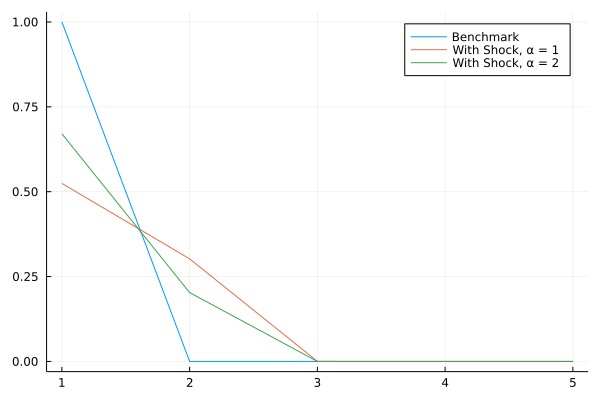
\includegraphics[width=0.8\textwidth]{decision_rules_c_f_10.png}
	\label{figure1}
\end{figure}

\begin{figure}[!htbp]
	\centering
	\caption{Decision Rules with Fixed Cost of Entry = 15}
	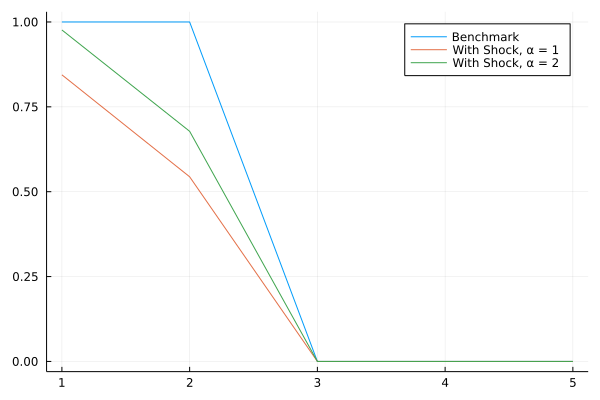
\includegraphics[width=0.8\textwidth]{decision_rules_c_f_15.png}
	\label{figure2}
\end{figure}



\end{document}

